\chapter{Revisão da literatura}
\label{chap:revisao}

\section{Gêmeo Digital}
\label{sec:digitaltwin}

O conceito de Gêmeos Digitais tem recebido considerável atenção acadêmica e industrial nas últimas duas décadas, consolidando-se como uma das principais tecnologias impulsionadoras da Indústria 4.0 \cite{dtchallenges, lu2020digitaltwin}. \citeonline{laessgen2012} descrevem o Gêmeo Digital como uma simulação multifísica, multiescala e probabilística integrada de um sistema complexo. Segundo os autores, essa tecnologia utiliza os melhores modelos físicos disponíveis e atualizações contínuas de sensores para espelhar a vida de seu correspondente físico de forma fiel.

A ideia fundacional dessa tecnologia foi introduzida pública e formalmente em 2003 por Michael Grieves, na Universidade de Michigan \cite{grieves2014, tao2019}. Segundo \citeonline{grieves2014}, a autoria do termo "Gêmeo Digital"\ pertence a John Vickers, da NASA, com quem Grieves colaborava na época. Em sua origem, as representações digitais possuíam um baixo nível de maturidade, frequentemente envolvendo a coleta manual e baseada em papel de informações do produto físico. Foi a partir da década seguinte, especialmente após 2010 e sob forte influência dos estudos da agência espacial americana, que o conceito experimentou uma evolução expressiva. O avanço das tecnologias da informação e a crescente disponibilidade de sensores físicos não destrutivos aumentaram de forma exponencial a quantidade, a riqueza e a fidelidade das informações \cite{grieves2014, tao2019}.

Inicialmente, a comunidade técnica interpretava o Gêmeo Digital apenas como um nível avançado de simulação tridimensional preliminar. Contudo, a literatura recente aponta que a simulação clássica é apenas um fragmento do ecossistema de um Gêmeo Digital. A principal característica que distancia o Gêmeo Digital da simulação computacional tradicional é a via de dados bidirecional e em tempo real \cite{sapandanylogic}. Enquanto modelos de simulação operam, na maioria das vezes, em ambientes estáticos e de forma \textit{offline}, o Gêmeo Digital exige uma conexão de alta fidelidade com o ativo físico, refletindo seu estado atual dinamicamente. 

Nesse sentido, a integração do Gêmeo Digital com todo o ciclo de vida do produto ou processo é considerada uma área de pesquisa promissora e em expansão \cite{sapandanylogic}. Um sistema fundamentado em Gêmeo Digital transcende a modelagem básica; ele engloba o monitoramento, a otimização e o controle do sistema real, demonstrando que um Gêmeo Digital é, em sua essência, muito mais do que apenas uma simulação.

Para além da sua definição conceitual, a arquitetura de um Gêmeo Digital é sustentada por núcleos fundamentais de funcionamento. Segundo \citeonline{tao2019}, um gêmeo digital opera através da interação estruturada de quatro elementos principais: Modelos, Dados, Conexões e Serviços. Os modelos atuam como contrapartes digitais que acompanham o ativo físico, possuindo funções que variam desde a reprodução de comportamentos em alta fidelidade até a previsão autônoma de problemas no espaço físico. Os dados, originados tanto no ambiente físico quanto no virtual, são o motor que impulsiona o Gêmeo Digital, permitindo a sua operação contínua e em tempo real. As conexões estabelecem o fluxo integrado de informações e garantem a sincronia em circuito fechado entre os espaços. Por fim, os serviços encapsulam a complexidade do sistema, fornecendo as respostas através de interfaces acessíveis aos utilizadores.




\section{Simulação Híbrida}
\label{sec:hibsim}

De acordo com \citeonline{mustafee2015}, a Simulação Híbrida  é a aplicação conjunta de técnicas de forma integrada, onde ambas as abordagens aprimoram harmoniosamente as capacidades uma da outra e reduzem limitações através do compartilhamento de informações. Na prática, a Simulação Híbrida busca obter sinergia. Por exemplo, enquanto a DES é mais adequada para modelar questões de foco operacional, ela pode ser combinada com outras técnicas baseadas em agentes para abranger problemas complexos de ponta a ponta \cite{fakhimi2023}.

No escopo do desenvolvimento de modelos, a Simulação Híbrida viabiliza a integração de métodos oriundos de diferentes disciplinas científicas, superando as barreiras entre a Pesquisa Operacional e a Ciência da Computação \cite{mustafee2015}. Nesse contexto, ganha destaque a combinação sinérgica entre a DES e a ABM. Essa integração torna-se estritamente necessária para a indústria da construção civil, uma vez que os projetos são altamente complexos e dinâmicos. Eles envolvem tanto o rigoroso fluxo logístico e sequencial das atividades e recursos (melhor representados pela DES) quanto o comportamento autônomo, interativo e estocástico dos operários no canteiro de obras (melhor representado pela ABM) \cite{fakhimi2023}. Ao unir essas duas abordagens, a Simulação Híbrida permite capturar simultaneamente as restrições técnicas e os fatores humanos do sistema de maneira coesa. 

Apesar da clara necessidade de lidar com essa complexidade mista, a aplicação da Simulação Híbrida na construção civil ainda se mantém esporádica, sendo implementada de forma mais pragmática do que sistemática \cite{fakhimi2023}. Uma revisão recente aponta que apenas cerca de 9\% das aplicações globais de Simulação Híbrida são direcionadas à construção \cite{fakhimi2023}. Dada a ampla utilização da simulação tradicional na indústria, esse baixo nível de adoção de modelos híbridos torna imperativo o desenvolvimento de novas pesquisas e soluções tecnológicas integradas para o setor \cite{fakhimi2023}.

\subsection{Simulação a Eventos Discretos (DES)}
\label{sec:DE}

Embora a nomenclatura seja semelhante, é fundamental não confundir a DES (Simulação a Eventos Discretos) com a teoria matemática de SED (Sistemas a Eventos Discretos), que será abordado nos próximos tópicos. Enquanto a formulação de SED foca na validação lógica e no sequenciamento formal de estados, a DES é amplamente utilizada na indústria e na academia como uma ferramenta computacional e analítica de apoio à decisão, capaz de simular a dinâmica de sistemas do mundo real evento por evento \cite{babulak2010}. Conforme destaca a literatura \cite{hybridframework}, a DES é essencialmente quantitativa e com mudanças discretas, sendo a abordagem mais adequada para modelar questões de foco operacional, como o tempo de ciclo e a alocação de recursos. Na prática, o desempenho do sistema é estruturado na simulação como uma sequência cronológica ao longo do tempo, em que cada ocorrência representa uma mudança brusca de estado no sistema \cite{zamani2024}.

Em relação a seu desempenho, a DES provou ser uma ferramenta eficaz por permitir reproduzir as interações entre recursos e atividades em cenários que envolvem fluxos físicos de materiais e componentes, como aponta \citeonline{babulak2010}. No contexto da execução de paredes de concreto, a abordagem orientada a eventos permite uma representação detalhada de fluxos de trabalho estritamente sequenciais, como a movimentação dos trabalhadores nas etapas de montagem e desmontagem. Ao lidar adequadamente com mudanças dinâmicas e incertezas temporais, a DES facilita o planejamento e a tomada de decisão gerencial por meio da análise iterativa de cenários \cite{zamani2024}.

Contudo, a aplicação isolada da DES na construção civil apresenta gargalos operacionais. Segundo \citeonline{zamani2024}, as simulações baseadas em eventos discretos possuem limitações significativas de visualização, uma vez que os softwares comerciais carecem das ferramentas visuais extensivas exigidas na gestão do canteiro de obras. Para superar essa limitação, uma solução plausível é a integração da DES com plataformas de representação visual. 

\subsection{Modelagem Baseada em Agentes (ABM)}
\label{sec:ABM}

A Modelagem Baseada em Agentes (ABM), assim como a DES, também atua sob a perspectiva de sistemas discretos, mas configura-se como uma abordagem computacional focada em entidades descentralizadas, sendo altamente adequada para os ciclos de monitoramento e controle em Gêmeos Digitais na construção \cite{sacks2020}. De acordo com \citeonline{bianchi2015}, a ABM simula a interação entre agentes heterogêneos inseridos em estruturas sociais complexas, como é o caso de um canteiro de obras.

Sendo uma abordagem relativamente nova para observar efeitos coletivos, a premissa central dessa técnica é que padrões globais emergem a partir de regras locais, sem que o comportamento final seja explicitamente programado \cite{mustafee2015}. Para estruturar essa modelagem, \cite{macal2005} definem três elementos constituintes de um ABM típico: (1) os agentes, dotados de atributos e comportamentos próprios; (2) os métodos de relacionamento e interação entre os agentes; e (3) a interação do agente com o seu ambiente.

Enquanto a DES gerencia a fila e os recursos logísticos, a ABM foca no indivíduo \cite{mustafee2015}. Em um canteiro de obras, a ABM permite representar os operários como agentes inteligentes com regras próprias de decisão e movimentação. Isso possibilita capturar as variabilidades humanas, o estresse e a maneira como as equipes interagem com as fôrmas, com o espaço físico reduzido e com outros trabalhadores, gerando uma representação computacional muito mais fiel da natureza imprevisível e dinâmica do trabalho manual nas obras \cite{mustafee2015}.

\section{Ferramentas Computacionais}
\label{sec:ferramentas}

A implementação de uma arquitetura de Gêmeo Digital baseada em Simulação Híbrida e Diagnose de Falhas exige a integração de plataformas de software robustas. Nesta seção, descrevem-se as principais ferramentas selecionadas para compor o ecossistema tecnológico deste trabalho, justificando suas adoções com base na literatura e nos requisitos do projeto.

\subsection{AnyLogic}
\label{subsec:anylogic}

O AnyLogic é reconhecido como a ferramenta pioneira na modelagem e simulação multimétodo, permitindo o desenvolvimento de modelos por meio da integração dos três principais métodos modernos de simulação: DES, ABM e Dinâmica de Sistemas (SD) \cite{AnyLogicFeatures}. 

\begin{figure}[!htb]
\centering
\caption{Métodos de simulação do Anylogic}
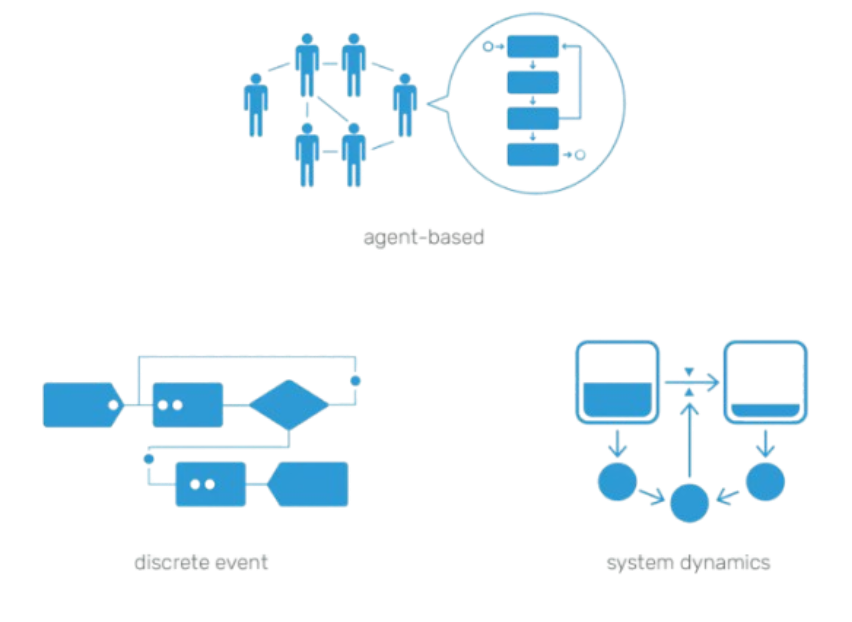
\includegraphics[width=0.8\textwidth]{Caps/Figs/anylogicModels.png}
\fonte{\citeonline{AnyLogicFeatures}}
\label{fig:anylogic-models}
\end{figure}
\FloatBarrier
Segundo \citeonline{AnyLogicFeatures}, esses métodos podem ser utilizados em qualquer combinação dentro de um único software, capacitando a plataforma a simular sistemas operacionais e de negócios de qualquer nível de complexidade, o que a torna uma base flexível e robusta para o desenvolvimento e experimentação de Gêmeos Digitais. Além disso, a ferramenta se destaca por oferecer diversas linguagens de modelagem visual, incluindo fluxogramas de processo, diagramas de estoque e fluxo, gráficos de ação e gráficos de estado (statecharts).

No escopo da construção civil, a escolha dessa ferramenta é amplamente respaldada pela literatura acadêmica. De acordo com a recente revisão conduzida por \citeonline{fakhimi2023}, o AnyLogic desponta como o software mais utilizado globalmente para a construção de modelos de Simulação Híbrida no setor, estando presente em grande parte dos estudos documentados na área. Além de facilitar a automação integrada entre diferentes pacotes, a ferramenta apresenta um alto nível de validação e verificação, sendo amplamente alimentada por dados do mundo real em projetos de construção \cite{fakhimi2023}.

Neste trabalho, o AnyLogic será a parte analítica do sistema. Ele será responsável não apenas por rodar a simulação logística das fôrmas (DES) e o comportamento dos operários (ABM), mas também por abrigar a lógica customizada dos Autômatos. A linguagem de programação utilizada para a personalização da lógica implementada no software foi a linguagem Java 17.

\subsection{NVIDIA Omniverse}
\label{subsec:omniverse}

O NVIDIA Omniverse é uma coleção de bibliotecas e microsserviços voltada para o desenvolvimento de aplicações, como gêmeos digitais industriais e simulações complexas \cite{NvidiaOmniverse}. Aproveitando a expertise da NVIDIA em computação acelerada, a plataforma integra funcionalidades avançadas, como bibliotecas de cálculo estrutural (NVIDIA PhysX) e renderização baseada em física e em tempo real (NVIDIA RTX). Fundamentado no padrão OpenUSD (Universal Scene Description), o Omniverse permite a interoperabilidade perfeita de dados e a colaboração em tempo real, viabilizando a criação de gêmeos digitais prontos para simulação.

\begin{figure}[!htb]
	\centering
	\caption{Exemplo de Gêmeo Digital no Nvidia Omniverse}
	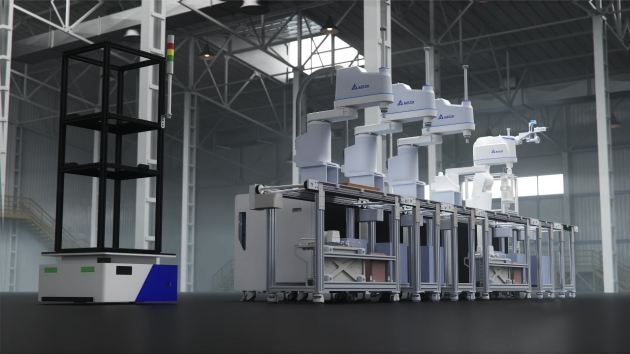
\includegraphics[width=0.8\textwidth]{Caps/Figs/omniverse.png}
	\fonte{\citeonline{NvidiaOmniverse}}
	\label{fig:omniverse-example}
\end{figure}
\FloatBarrier
Conforme discutido anteriormente com base em \citeonline{zamani2024}, os softwares comerciais voltados para simulação apresentam limitações significativas de visualização, carecendo das ferramentas gráficas e espaciais extensivas exigidas na gestão prática de um canteiro de obras. Sendo assim, o Omniverse foi selecionado para preencher exatamente essa lacuna tecnológica. Neste projeto, o Omniverse atuará como a interface de visualização do Gêmeo Digital. Ele receberá os dados processados gerados em tempo real pelo AnyLogic, traduzindo essas informações analíticas em uma representação geométrica tridimensional e interativa do canteiro. 
 
\section{Sistemas a Eventos Discretos (SED)}
\label{sec:sed}

Os SED são sistemas dinâmicos de estados discretos cuja transição se dá por meio da ocorrência, em geral assíncrona, de eventos \cite{ basilio2010}. O fato de o estado do sistema ser discreto implica que este pode assumir valores simbólicos, como por exemplo \{ligado, desligado\}, ou valores numéricos pertencentes a conjuntos discretos (como $\mathbb{N}$ ou $\mathbb{Z}$). Os eventos, por sua vez, podem estar associados a ações específicas iniciadas por agentes ou ser o resultado do cumprimento de diversas condições lógicas ou físicas\cite{ basilio2010}.

Embora seja possível modelar praticamente qualquer sistema físico como um SED, dependendo do grau de abstração adotado, determinados ambientes operacionais são naturalmente discretos e têm sua evolução determinada estritamente pela ocorrência de eventos \cite{mestradoDudu}. Nesse sentido, as etapas de trabalho em um canteiro de obras enquadram-se perfeitamente nesse paradigma, uma vez que o avanço físico da montagem ou desmontagem de formas dependem de transições pontuais e sequenciais do processo de construção.

Ao se considerar a evolução de um SED, a maior preocupação da modelagem reside na sequência de estados visitados e nos eventos que causaram as correspondentes transições \cite{mestradoDudu}. Conforme fundamentado pela teoria clássica de \cite{cassandra2008}, o modelo formal de um SED é composto basicamente por esses dois elementos fundamentais: Estados e Eventos.

\subsection{Estados e Eventos}
\label{subsec:estados_eventos}

O Estado de um sistema num instante deve descrever o seu comportamento
nesse instante de alguma forma mensurável \cite{cassandra2008}. Ele funciona como a memória do sistema naquele momento, assumindo valores discretos e simbólicos. No contexto de um canteiro de obras, cada processo da montagem ou desmontagem de uma forma pode ser definido como um Estado.

Os Eventos, por sua vez, são as ocorrências instantâneas responsáveis por causar a transição do sistema de um estado para outro \cite{cassandra2008}. Um Evento pode estar associado a uma ação específica iniciada por um agente ou ser o resultado do cumprimento de uma condição física no sistema. A evolução de um SED é ditada estritamente pela sequência em que esses Eventos ocorrem \cite{basilio2010}.

\subsection{Eventos Observáveis, Não Observáveis e a Diagnose de Falhas}
\label{subsec:observabilidade_falhas}

Para que seja possível aplicar a teoria de SED na identificação de problemas reais, é necessário classificar os eventos do sistema de acordo com a sua capacidade de serem registados. Segundo \citeonline{basilio2010}, a diagnose de falhas em SEDs é norteada por dois paradigmas centrais:
\begin{enumerate}
	\item As falhas a serem diagnosticadas são inerentemente Eventos Não Observáveis, isto é, são ocorrências que não podem ser diretamente registadas por sensores físicos ou por apontamentos diretos no canteiro de obras;
	\item A ocorrência de uma falha altera o comportamento do sistema, porém não leva necessariamente à sua paragem imediata. Por exemplo, a ocorrência de uma falha não diagnosticada em um processo de manufatura ou construção civil pode levar apenas a uma degradação invisível dos indicadores de eficácia global, como atrasos logísticos ou queda de qualidade \cite{basilio2010}.
\end{enumerate}

Dessa forma, o problema da diagnose de falhas consiste em inferir a ocorrência de um evento de falha não observável baseando-se exclusivamente no histórico dos eventos regulares que foram Observáveis. De maneira informal, diz-se que um evento de falha pode ser diagnosticado se a sua ocorrência puder ser detetada com exatidão após a ocorrência de um número finito de Eventos Observáveis subsequentes \cite{basilio2010}.

Para atingir esse objetivo, constroem-se sistemas de diagnose de falhas atuando como "sensores virtuais". O projeto destes sistemas requer a construção prévia de um SED que capture tanto o comportamento normal quanto o comportamento falho do sistema \cite{basilio2010}.

\subsection{Autômatos Finitos Determinísticos ($G$)}
\label{subsec:automatos}

Uma das maneiras mais eficientes e rigorosas de se modelar e visualizar um SED é através de Autômatos Finitos Determinísticos. Um autômato é um dispositivo matemático capaz de representar a linguagem de um sistema de acordo com regras bem definidas, sendo frequentemente ilustrado por diagramas de transição de estados \cite{basilio2010}.


\begin{figure}[!htb]
	\centering
	\caption{Exemplo de Autômato}
	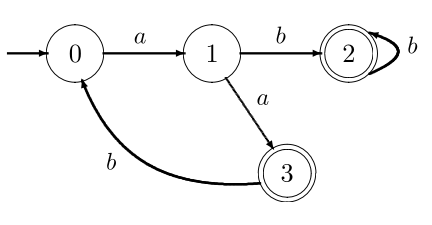
\includegraphics[width=0.6\textwidth]{Caps/Figs/automato.png}
	\fonte{\citeonline{basilio2010}}
	\label{fig:exemplo-automato}
\end{figure}

\FloatBarrier

Formalmente, um autômato determinístico é definido pela quíntupla:
\begin{equation}
	G = (X, \Sigma, f, x_0, X_m)
\end{equation}
onde:
\begin{itemize}
	\item $X$ é o conjunto finito de estados do sistema;
	\item $\Sigma$ é o conjunto finito de eventos (alfabeto);
	\item $f: X \times \Sigma \to X$ é a função de transição parcial, que define o novo estado do sistema após a ocorrência de um evento;
	\item $x_0 \in X$ é o estado inicial do sistema;
	\item $X_m \subseteq X$ é o subconjunto de estados marcados (geralmente associados à conclusão de tarefas ou ciclos operacionais).
\end{itemize}

Para complementar a dinâmica do modelo, define-se $\Gamma(x) \subseteq \Sigma$ como o conjunto de Eventos ativos no estado $x$, ou seja, o subconjunto de eventos que estão fisicamente ou logicamente habilitados a ocorrer quando o sistema se encontra naquele estado específico.

Para que seja possível aplicar a teoria de diagnose de falhas sobre o modelo $G$, a literatura clássica estabelece três premissas fundamentais que o sistema deve respeitar \cite{basilio2010}. No contexto da modelagem logística de um canteiro de obras, essas hipóteses traduzem-se da seguinte forma:

\begin{enumerate}
	\item \textbf{A1 - Sistema Vivo ($\Gamma(x) \neq \emptyset$ para todo $x \in X$):} Assume-se que o autômato gerado por $G$ não possui Estados de travamento irreversível (deadlocks). Na prática, isso significa que a obra está em contínua operação, mesmo que ocorra uma falha logística ou um atraso, o sistema sempre terá algum Evento possível para dar sequência ao processo.
	\item \textbf{A2 - Ausência de ciclos não Observáveis:} O modelo não pode possuir nenhum ciclo de estados formado exclusivamente por Eventos Não Observáveis. Essa hipótese garante que, caso uma falha oculta ocorra, o sistema não ficará preso em um \textit{loop} invisível aos sensores. O processo de construção continuará avançando até gerar um evento observável, permitindo que o Gêmeo Digital detecte a falha pregressa.
	\item \textbf{A3 - Único tipo de falha ($\Sigma_f = \{\sigma_f\}$):} Embora tutoriais clássicos muitas vezes assumam um único tipo de falha por simplicidade didática, a teoria permite a modelagem de múltiplos eventos anômalos. Para isso, o conjunto de falhas $\Sigma_f$ é particionado em $m$ classes disjuntas. No escopo deste trabalho, o sistema contemplará diferentes tipos de falha (como, por exemplo, problemas na montagem ou atrasos na concretagem), sendo os fundamentos de diagnosticabilidade aplicados para identificar a ocorrência de cada classe de falha de maneira independente 
\end{enumerate}


\subsection{Diagnose Centralizada sob Observação Parcial}
\label{subsec:diagnosticador}

A essência da diagnose de falhas em um SED reside na capacidade de inferir a ocorrência de Eventos Não Observáveis a partir da sequência de Eventos Observáveis gerada pelo sistema. Para formalizar essa restrição de visibilidade, define-se o conjunto de eventos do sistema como a união disjunta $\Sigma = \Sigma_o \cup \Sigma_{uo}$, onde $\Sigma_o$ representa os Eventos Observáveis (registrados pelos sensores ou apontamentos no canteiro) e $\Sigma_{uo}$ os Eventos Não Observáveis (que incluem o subconjunto de eventos de falha $\Sigma_f$). 

Para que a tomada de decisão sobre a ocorrência ou não de uma falha seja realizada por um único agente analítico, utiliza-se a abordagem de diagnose centralizada. O projeto desse agente é dividido metodologicamente em duas etapas de modelagem: o Autômato Rotulador ($G_{al}$) e o Autômato Diagnosticador ($G_d$).



\subsubsection{Autômato Rotulador ($G_{al}$)}

Para rastrear o impacto das falhas ao longo das transições do sistema, o primeiro passo consiste na construção de um Autômato Rotulador ($G_{al}$). Este autômato expande o modelo original $G$, acoplando ao estado físico do sistema uma "etiqueta" (ou rótulo) que indica a ocorrência de anomalias. Define-se o conjunto de rótulos $\Delta = \{N, F_1, F_2\}$, onde $N$ indica o comportamento Normal, enquanto $F_1$ e $F_2$ indicam a ocorrência pregressa das respectivas classes de falha modeladas na obra.

\begin{figure}[!htb]
	\centering
	\caption{Exemplo de Autômato Rotulador}
	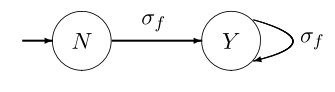
\includegraphics[width=0.6\textwidth]{Caps/Figs/rotulador.png}
	\fonte{\citeonline{basilio2010}}
	\label{fig:exemplo-rotulador}
\end{figure}

\FloatBarrier
Dessa forma, os estados do autômato rotulador assumem a forma de pares ordenados $(x, l)$, onde $x \in X$ é o estado da planta e $l \in \Delta$ é a condição de falha associada. O $G_{al}$ processa todos os Eventos (Observáveis e Não Observáveis). Quando um evento de falha ocorre, o autômato altera o rótulo de $N$ para $F_i$ e propaga essa etiqueta para todos os Estados subsequentes, funcionando como uma memória permanente de que o sistema foi corrompido.

\subsection{Composição Paralela}

A operação de composição paralela é fundamental na teoria de SED quando se deseja modelar o comportamento conjunto e interativo de múltiplos subsistemas \cite{mestradoDudu}. Segundo \cite{basilio2010}, essa operação estabelece as regras de sincronização entre dois autômatos, definindo como os eventos comuns e os eventos privados devem se comportar.

Suponha dois autômatos distintos definidos por $G_1 = (X_1, \Sigma_1, f_1, \Gamma_1, x_{01}, X_{m1})$ e $G_2 = (X_2, \Sigma_2, f_2, \Gamma_2, x_{02}, X_{m2})$. O autômato resultante que modela o comportamento síncrono de $G_1$ e $G_2$ é obtido através da composição paralela, denotada por $G_1 \parallel G_2$. Nesse novo modelo, duas regras fundamentais de execução são estabelecidas:
\begin{itemize}
	\item \textbf{Eventos comuns:} Um evento pertencente a ambos os alfabetos ($\sigma \in \Sigma_1 \cap \Sigma_2$) somente poderá ocorrer de forma sincronizada, ou seja, quando ambos os autômatos estiverem em estados cujos conjuntos de Eventos ativos possuam esse Evento de forma simultânea.
	\item \textbf{Eventos privados:} Eventos pertencentes exclusivamente a um dos sistemas, definidos matematicamente por $\Sigma_1 \setminus \Sigma_2$ ou $\Sigma_2 \setminus \Sigma_1$, não requerem sincronização e podem ser executados de forma independente sempre que estiverem ativos no seu respectivo autômato.
\end{itemize}

Formalmente, a composição paralela de $G_1$ e $G_2$ é definida pela seguinte estrutura:
$$G_1 \parallel G_2 = Ac(X_1 \times X_2, \Sigma_1 \cup \Sigma_2, f_{1 \parallel 2}, \Gamma_{1 \parallel 2}, (x_{01}, x_{02}), X_{m1} \times X_{m2})$$

onde $\times$ denota o produto cartesiano e $Ac(\cdot)$ representa a operação que extrai a parte acessível do autômato, filtrando e mantendo apenas os estados que podem ser alcançados a partir do estado inicial $(x_{01}, x_{02})$ por meio de uma sequência válida de eventos em $(\Sigma_1 \cup \Sigma_2)^*$.

A evolução da dinâmica desse sistema composto é governada pela sua função de transição parcial, $f_{1 \parallel 2} : (X_1 \times X_2) \times (\Sigma_1 \cup \Sigma_2) \to (X_1 \times X_2)$, definida por \cite{basilio2010} da seguinte forma:
$$f_{1 \parallel 2}((x_1, x_2), \sigma) = \begin{cases}
	(f_1(x_1, \sigma), f_2(x_2, \sigma)), & \text{se } \sigma \in \Gamma_1(x_1) \cap \Gamma_2(x_2) \\
	(f_1(x_1, \sigma), x_2), & \text{se } \sigma \in \Gamma_1(x_1) \setminus \Sigma_2 \\
	(x_1, f_2(x_2, \sigma)), & \text{se } \sigma \in \Gamma_2(x_2) \setminus \Sigma_1
\end{cases}$$



\subsection{Autômato Observador}

O comportamento dinâmico de um autômato que possui Eventos Não Observáveis pode ser descrito por um novo autômato determinístico, denominado \textit{Observador}, cujo conjunto de eventos é formado exclusivamente pelos Eventos Observáveis do sistema original. Os Estados do Observador correspondem a todos os Estados possíveis em que o autômato com Eventos Não Observáveis poderia estar após a ocorrência de uma dada sequência de Eventos Observáveis \cite{basilio2010}.

O Observador para um autômato $G$, denotado por $Obs(G)$, é formalmente definido pela seguinte quíntupla:
$$Obs(G) = (X_{obs}, \Sigma_{obs}, f_{obs}, \Gamma_{obs}, x_{0,obs}, X_{m,obs})$$

sendo que o conjunto de Estados do Observador pertence ao conjunto das partes de $X$, isto é, $X_{obs} \subseteq 2^X$. Os Estados marcados do Observador são definidos como $X_{m,obs} = \{q \in X_{obs} : q \cap X_m \neq \emptyset\}$. 

Para a definição formal do estado inicial $x_{0,obs}$, da função de Eventos ativos $\Gamma_{obs}$ e da função de transição $f_{obs}$, é necessário introduzir o conceito de \textbf{Alcance Não-Observável} (\textit{Unobservable Reach}). O Alcance Não Observável de um Estado $x \in X$, denotado por $UR(x)$, é o conjunto de Estados que podem ser alcançados a partir de $x$ por meio da ocorrência exclusiva de Eventos Não Observáveis:
$$UR(x) = \{x' \in X : (\exists s \in \Sigma_{uo}^*)[f(x, s) = x']\}$$

De forma análoga, o Alcance Não Observável de um subconjunto de Estados $q \in 2^X$ é definido como a união dos alcances individuais de cada Estado contido em $q$:
$$UR(q) = \bigcup_{x \in q} UR(x)$$

Utilizando essas definições, os elementos de $Obs(G)$ podem ser construídos sistematicamente por meio do algoritmo da Figura \ref{fig:algoritmoobservador}.
\begin{figure}[!htb]
	\centering
	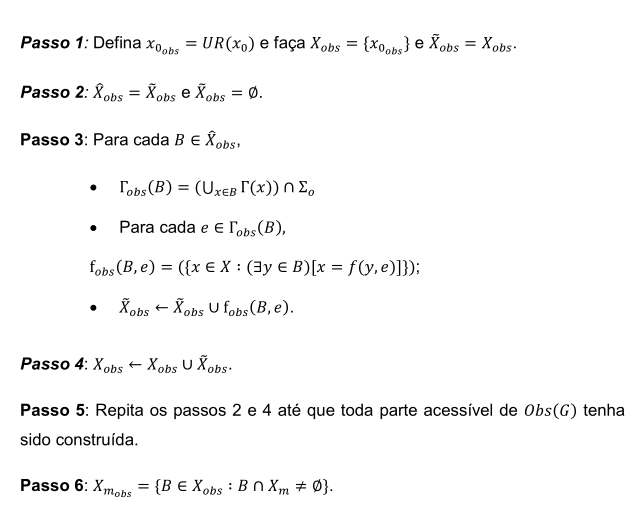
\includegraphics[width=0.7\linewidth]{Caps/Figs/algoritmoObservador}
	\caption{Algoritmo de construção do Autômato Observador}
	\fonte{\cite{mestradoDudu}}
	\label{fig:algoritmoobservador}
\end{figure}
\FloatBarrier

A lógica fundamental desse algoritmo consiste em calcular o alcance não observável para cada Estado de $G$ que é atingido logo após a ocorrência de um evento Observável. Assim, no Passo 1, calcula-se o Alcance Não Observável do estado inicial $x_0$, formando o Estado inicial do Observador. No Passo 3, determinam-se os Eventos ativos dos Estados do Observador obtidos na iteração anterior. Além disso, calculam-se os próximos Estados do Observador, que correspondem aos Alcances Não Observáveis dos Estados de $G$ atingidos a partir do Estado atual do Observador por meio de Eventos Observáveis. Essa sequência iterativa é repetida até que todos os Estados acessíveis do Observador tenham sido mapeados (Cassandras e Lafortune, 2008).


\subsubsection{Autômato Diagnosticador ($G_d$)}


O diagnosticador centralizado, comumente denotado por $G_d$, é um autômato construído especificamente para realizar o rastreamento de falhas do sistema em tempo real. O seu conjunto de Eventos é estritamente igual ao conjunto dos Eventos Observáveis do modelo da planta $G$. A principal característica do diagnosticador é que seus estados são formados pela adição de rótulos (tipicamente $N$ (\textit{Normal}) e $F$ (\textit{Falha})) aos Estados originais de $G$, com o objetivo de indicar se um determinado Evento de falha Não Observável ($\sigma_f$) já ocorreu ou não.

Formalmente, o diagnosticador $G_d$ é definido pela seguinte estrutura de autômato:
$$G_d = (X_d, \Sigma_d, f_d, \Gamma_d, x_{0,d}, X_{m,d})$$

sendo que o espaço de Estados do diagnosticador é um subconjunto das partes do produto cartesiano entre os Estados do sistema e o conjunto de rótulos, isto é, $X_d \subseteq 2^{X \times \{N, F\}}$. O conjunto de Eventos ativos no diagnosticador corresponde unicamente aos Eventos Observáveis do sistema ($\Sigma_d = \Sigma_{obs}$).

A síntese matemática do diagnosticador $G_d$ pode ser realizada de forma sistemática por meio de dois passos operacionais fundamentais:
\begin{enumerate}
	\item[(i)] Obtenha a composição paralela $G \parallel A_l$, sendo $A_l$ o autômato rotulador de dois Estados, projetado para alterar seu Estado de "Normal" para "Falha" irreversivelmente após a ocorrência de $\sigma_f$, conforme ilustrado na Figura \ref{fig:automato_rotulador};
	\item[(ii)] Calcule o autômato Observador para essa composição paralela gerada no passo anterior, ou seja, construa $Obs(G \parallel A_l)$ utilizando o Algoritmo de Alcance Não Observável previamente definido.
\end{enumerate}

\begin{figure}[!htb]
	\centering
	\caption{Exemplo de construção de um autômato diagnosticador $G_d$.}
	
	\begin{minipage}{0.34\textwidth}
		\centering
		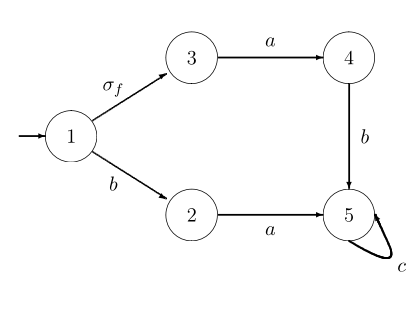
\includegraphics[width=\textwidth]{Caps/Figs/automatoBasilio.png}
		\caption*{(a) Exemplo de Autômato G.}
		\label{fig:automatoG}
	\end{minipage}
	\hfill
	\begin{minipage}{0.32\textwidth}
		\centering
		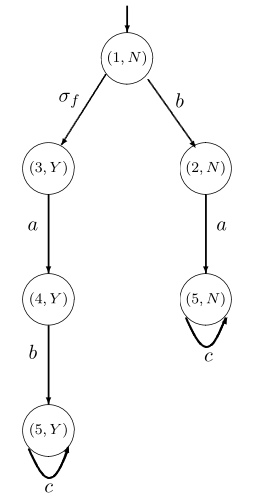
\includegraphics[width=\textwidth]{Caps/Figs/composicaoParalela.png}
		\caption*{(b) Composição paralela entre $G$ e $A_l$.}
		\label{fig:composicaoParalela}
	\end{minipage}
	\hfill
	\begin{minipage}{0.32\textwidth}
		\centering
		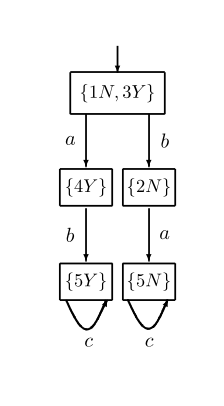
\includegraphics[width=\textwidth]{Caps/Figs/observador.png}
		\caption*{(c) $G_d = Obs(G \parallel A_l)$.}
		\label{fig:observador}
	\end{minipage}
	
	\fonte{\citeonline{basilio2010}.}
	
\end{figure}
\FloatBarrier


\subsection{Diagnosticabilidade}
\label{subsec:diagnosticabilidade}

A construção de um Autômato Diagnosticador ($G_d$) não garante, por si só, que todas as anomalias do sistema serão invariavelmente identificadas. Para que o monitoramento seja efetivo e o sensor virtual funcione, a linguagem gerada pelo sistema deve possuir uma propriedade fundamental denominada Diagnosticabilidade \cite{basilio2010}.

De maneira informal, diz-se que a linguagem gerada por um autômato é Diagnosticável em relação a um conjunto de Eventos Observáveis $\Sigma_o$ e a uma classe de falhas $\Sigma_f$ se a ocorrência de um evento de falha puder ser detectada com exatidão após um número finito de transições subsequentes, utilizando exclusivamente a leitura das sequências de Eventos Observáveis \cite{basilio2010}.

Na prática da modelagem de um canteiro de obras, isso significa que, após a ocorrência de uma anomalia oculta, o processo logístico deve obrigatoriamente continuar avançando e gerando eventos visíveis suficientes para que o Gêmeo Digital deduza a falha pregressa. O sucesso desse processo ocorre quando o autômato diagnosticador consegue sair de um estado de "Incerteza" e transitar definitivamente para um estado de "Certeza de Falha".

Por outro lado, um sistema é classificado como Não Diagnosticável quando existe a possibilidade de o diagnosticador ficar preso indefinidamente em estados de incerteza. Matematicamente, isso ocorre quando o modelo da planta possui ciclos de eventos que geram exatamente a mesma projeção observável tanto para um comportamento normal quanto para um comportamento falho. Diante dessa ambiguidade permanente, o sistema analítico torna-se incapaz de confirmar a ocorrência da anomalia, independentemente de quanto tempo o monitoramento continue. Nesses casos, a teoria de controle indica que o projeto do sistema deve ser revisto, seja adicionando novos sensores ou alterando a lógica do processo, para que a falha se torne detectável.



\section{Consideração do capítulo}

A compreensão do canteiro de obras, a análise do comportamento humano por meio da ABM e o fluxo físico da construção da parede de concreto realizada pela DES evidenciam uma realidade crítica: as decisões diárias dos trabalhadores são a causa raiz de diversos defeitos construtivos nas paredes de concreto. Essa dinâmica comportamental gera uma necessidade constante de retrabalho, o que compromete severamente a produtividade global e o planejamento da obra. A não execução de qualquer atividade essencial resulta, portanto, na consolidação de uma não conformidade.

Contudo, a simples observação física ou o uso de formulários de verificação tradicionais não são suficientes para capturar essas infrações, uma vez que elas ocorrem, na maioria das vezes, de forma silenciosa. O trabalhador burla os mecanismos de controle sem deixar rastros imediatos, o que faz com que esses erros se comportem, na ótica da simulação, como Eventos de Falha Não Observáveis.

É exatamente para solucionar essa lacuna de rastreabilidade percebida pela Simulação Híbrida que surge a necessidade da aplicação da teoria de Sistemas a Eventos Discretos (SED), cujo arcabouço lógico será detalhado nos próximos capítulos. O estudo do SED é uma alternativa para este trabalho porque permite avançar da simples constatação do problema para o diagnóstico formal. O mapeamento das atividades do canteiro servirá como base para a construção de um modelo capaz de rastrear o fluxo visível (Observável) da obra e inferir, matematicamente, a ocorrência dessas anomalias ocultas, conectando o comportamento operário à detecção analítica de falhas no processo produtivo.
 %Não consegui correlacionar com Gêmeos Digitais, falei de simulação hibrida aliada a SED
 
